\documentclass{article}
\usepackage[utf8]{inputenc}
\usepackage{array}
\usepackage{multicol}
\usepackage{listings}
\usepackage{amssymb}
\usepackage{enumitem}
\usepackage{graphicx}
\usepackage{amsthm}
\usepackage{hyperref}
\usepackage{tikz}
\usepackage{amssymb}
\usepackage{amsmath}
\usepackage{mathtools}

\usetikzlibrary{automata,positioning}

\begin{document}

\title{Talen \& Automaten \\ Assignment 3}
\date{\today}
\author{Tony Lopar \enspace s1013792 \\TA: Nienke Wessel}
\maketitle

\section*{Exercise 1}
A possible automate for this language is drawn in figure~\ref{Fig:M1}.
\begin{figure}[h]
\begin{center}
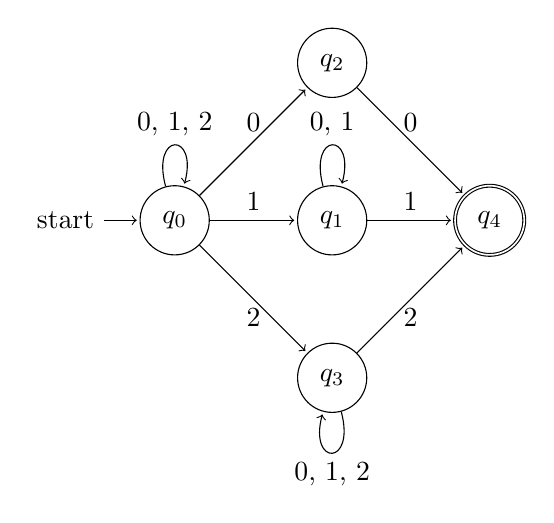
\begin{tikzpicture}[shorten >=1pt,node distance=2cm,on grid,auto]
   \node[state,initial] (q_0)   {$q_0$};
   \node[state] (q_1) [right=of q_0]  {$q_1$};
   \node[state](q_2) [above=of q_1] {$q_2$};
   \node[state](q_3) [below=of q_1] {$q_3$};
   \node[state,accepting](q_4) [right=of q_1] {$q_4$};
    \path[->]
    (q_0) edge [left]  node [above] {1} (q_1)
          edge [left]  node [above] {0} (q_2)
          edge [left]  node [below] {2} (q_3)
          edge [loop above] node  {0, 1, 2} ()
    (q_1) edge [loop above] node  {0, 1} ()
          edge [left]  node [above] {1} (q_4)
    (q_2) edge [left]  node [above] {0} (q_4)
    (q_3) edge [loop below] node  {0, 1, 2} ()
          edge [left]  node [below] {2} (q_4);
\end{tikzpicture}
\end{center}
  \caption{A possible automate for L from exercise 1} \label{Fig:M1}
\end{figure}

We may show that 2101 is accepted if we take a look at the transition function below. We see that the set of possible transition states at the end contains the accepting state $q_4$ which means the word is accepted.
\begin{align*}
  \delta^* (q_0, 2101)  &= \delta^* (\delta^*(q_0, 2), 101) &= \delta^* (\{q_0, q_3 \}, 101) \\
                        &= \delta^* (\delta^*(\{q_0, q_3 \}, 1), 01) &= \delta^* (\{q_0, q_1, q_3 \}, 01) \\
                        &= \delta^* (\delta^*(\{q_0, q_1, q_3 \}, 0), 1) &= \delta^* (\{q_0, q_1, q_2, q_3 \}, 1) \\
                        &= \delta^* (\delta^*(\{q_0, q_1, q_2, q_3 \}, 1), \lambda) &= \delta^* (\{q_0, q_1, q_2, q_3, q_4 \}, \lambda) \\
\end{align*}

We may show that 121 is not accepted since it isn't in the set of the possible end states of the word. We also see that $q_1$ is in the first part of the second equation and not in the second, since there is no path for the word 2 possible from $q_1$.
\begin{align*}
  \delta^* (q_0, 121)   &= \delta^* (\delta^*(q_0, 1), 21) &= \delta^* (\{q_0, q_1 \}, 21) \\
                        &= \delta^* (\delta^*(\{q_0, q_1 \}, 2), 1) &= \delta^* (\{q_0, q_3 \}, 1) \\
                        &= \delta^* (\delta^*(\{q_0, q_3 \}, 1), \lambda) &= \delta^* (\{q_0, q_3 \}, \lambda) \\
\end{align*}

\section*{Exercise 2}
The transformation we need to perform in the automate is that we need to remove the $\lambda$ paths and add paths to keep the language the same. First we make the states that can reach the accepting state $q_3$ with a $\lambda$ also accepting. This is the state $q_0$ in this case.

Furthermore, we have a $\lambda$-step between $q_1$ and $q_2$. We see that we can reach $q_2$ in the original automate with 'b,c' and possibly some a's. In order to keep both ways possble we split the paths into a path with only 'b,c' and a path where it has to be followed by one or more 'a'.
  % \begin{center}
  % \begin{tikzpicture}[shorten >=1pt,node distance=2cm,on grid,auto]
  %    \node[state,initial] (q_0)   {$q_0$};
  %    \node[state] (q_1) [right=of q_0]  {$q_1$};
  %    \node[state](q_2) [right=of q_1] {$q_2$};
  %    \node[state,accepting](q_3) [right=of q_2] {$q_3$};
  %     \path[->]
  %     (q_0) edge [left]  node [above] {b,c} (q_1)
  %           edge [bend left=60]  node  {$\lambda$} (q_3)
  %           edge [loop above] node  {a,b} ()
  %     (q_1) edge [loop above] node  {a} ()
  %           edge [left]  node [above] {$\lambda$} (q_2)
  %     (q_2) edge [loop above] node  {a, b, c} ()
  %           edge [left]  node [above] {c} (q_3);
  % \end{tikzpicture}
  % \end{center}

\begin{figure}[h]
\begin{center}
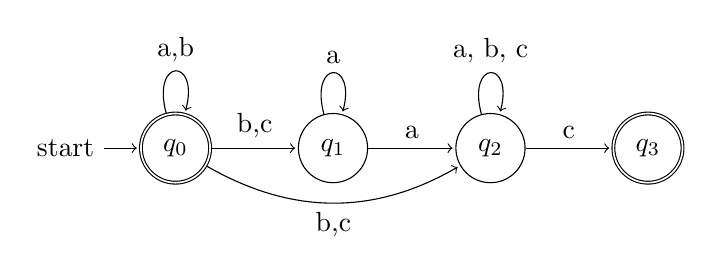
\begin{tikzpicture}[shorten >=1pt,node distance=2cm,on grid,auto]
   \node[state,initial, accepting] (q_0)   {$q_0$};
   \node[state] (q_1) [right=of q_0]  {$q_1$};
   \node[state](q_2) [right=of q_1] {$q_2$};
   \node[state,accepting](q_3) [right=of q_2] {$q_3$};
    \path[->]
    (q_0) edge [left]  node [above] {b,c} (q_1)
          edge [bend right]  node [below] {b,c} (q_2)
          edge [loop above] node  {a,b} ()
    (q_1) edge [loop above] node  {a} ()
          edge [left]  node [above] {a} (q_2)
    (q_2) edge [loop above] node  {a, b, c} ()
          edge [left]  node [above] {c} (q_3);
\end{tikzpicture}
\end{center}
  \caption{$NFA-\lambda$ to NFA} \label{Fig:M2}
\end{figure}

\section*{Exercise 3}
In order to convert this NFA to a DFA we should find out where all of the possible transitions should go and which are missing. First, we keep track of all states where we can go and we see that we can go into two directions from $q_1$ with a 'b'. This means that a 'b' should direct the subset with both states in the DFA.

Furthermore, we see that from $q_0$ 'b' doesn't points to a state. This means that the b isn't known in this state and points to the empty set.
\begin{figure}[h]
\begin{center}
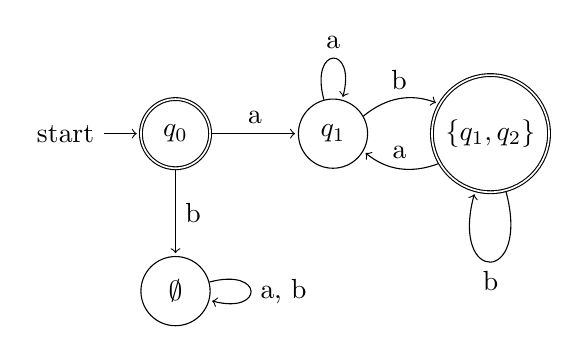
\begin{tikzpicture}[shorten >=1pt,node distance=2cm,on grid,auto]
   \node[state,initial, accepting] (q_0)   {$q_0$};
   \node[state] (q_1) [right=of q_0]  {$q_1$};
   \node[state, accepting](q_2) [right=of q_1] {$\{ q_1, q_2 \}$};
   \node[state](q_3) [below=of q_0] {$\emptyset$};
    \path[->]
    (q_0) edge [left]  node [above] {a} (q_1)
          edge [left]  node [right] {b} (q_3)
    (q_1) edge [loop above] node  {a} ()
          edge [bend left]  node [above] {b} (q_2)
    (q_2) edge [bend left]  node [above] {a} (q_1)
          edge [loop below] node  {b} ()
    (q_3) edge [loop right] node  {a, b} ();
\end{tikzpicture}
\end{center}
  \caption{NFA to DFA} \label{Fig:M3}
\end{figure}

\section*{Exercise 4}
The regular expression states that we have whether zero or multiple 'a's or a 'b' followed by one 'a'. Using the toolkit from the slides we start by making two lambda steps to the automata of both possibilities. Since the a of the loop may be executed zero or more times we may also pass it with the empty word.

Both options end in state $q_4$. After both options a second automate that's connected with a $\lambda$ needs an 'a' to result in the accepting state.

These described steps result in the following $NFA-\lambda$ of figure~\ref{Fig:M4}
\begin{figure}[h]
\begin{center}
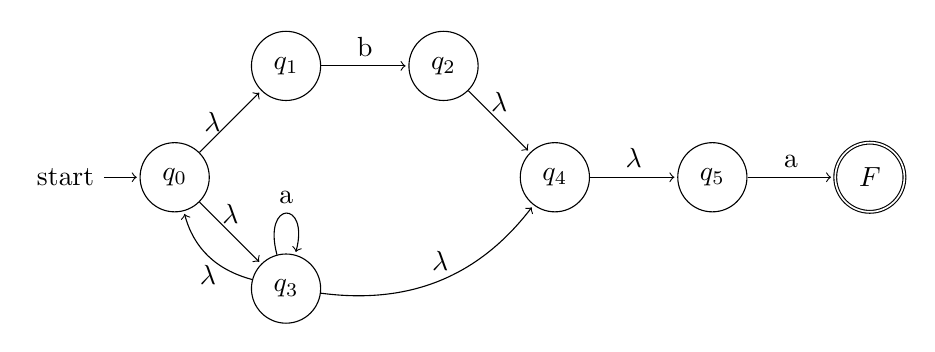
\begin{tikzpicture}[shorten >=1pt,node distance=2cm,on grid,auto]
   \node[state,initial] (q_0)   {$q_0$};
   \node[state] (q_1) [above right=of q_0]  {$q_1$};
   \node[state](q_2) [right=of q_1] {$q_2$};
   \node[state](q_3) [below right=of q_0] {$q_3$};
   \node[state](q_4) [below right=of q_2] {$q_4$};
   \node[state](q_5) [right of=q_4] {$q_5$};
   \node[state,accepting](F) [right=of q_5] {$F$};
    \path[->]
    (q_0) edge [left]  node  {$\lambda$} (q_1)
          edge [left]  node [above] {$\lambda$} (q_3)
    (q_1) edge [left]  node [above] {b} (q_2)
    (q_2) edge [left]  node [above] {$\lambda$} (q_4)
    (q_3) edge [loop above] node  {a} ()
          edge [bend right]  node [above] {$\lambda$} (q_4)
          edge [bend left]  node [below] {$\lambda$} (q_0)
    (q_4) edge [left]  node [above] {$\lambda$} (q_5)
    (q_5) edge [left]  node [above] {a} (F);
\end{tikzpicture}
\end{center}
  \caption{$NFA-\lambda$ of the reqex $(b + a^*)a$} \label{Fig:M4}
\end{figure}

\end{document}
